\documentclass{scrreprt}
\usepackage{listings}
\usepackage{underscore}
\usepackage{graphicx}
\usepackage[bookmarks=true]{hyperref}
\usepackage[utf8]{inputenc}
\usepackage[english]{babel}
\usepackage{array}
\usepackage{booktabs}

\hypersetup{
    bookmarks=false,    % show bookmarks bar?
    pdftitle={Software Requirement Specification},    % title
    pdfauthor={Jean-Philippe Eisenbarth},                     % author
    pdfsubject={TeX and LaTeX},                        % subject of the document
    pdfkeywords={TeX, LaTeX, graphics, images}, % list of keywords
    colorlinks=true,       % false: boxed links; true: colored links
    linkcolor=blue,       % color of internal links
    citecolor=black,       % color of links to bibliography
    filecolor=black,        % color of file links
    urlcolor=purple,        % color of external links
    linktoc=page            % only page is linked
}%
\def\myversion{1.0 }
\date{}
%\title
\usepackage{hyperref}
\begin{document}

\begin{flushright}
    \rule{16cm}{5pt}\vskip1cm
    \begin{bfseries}
        \Huge{SOFTWARE REQUIREMENTS\\ SPECIFICATION}\\
        \vspace{1cm}
        for\\
        \vspace{1cm}
        Crop and Fertilizer Recommendation System\\
        \vspace{1.5cm}
        \LARGE{Version \myversion}\\
        \vspace{1cm}
        Prepared by: 1. Mohanty Hitesh Rabindranath (2201298111)\\
        2. Syed Sadiqu Hussain \\(2201298227)\\
        \vspace{1cm}
        Submitted to: Biswadarsi Biswal  \\Lecturer\\
        \vspace{1cm}
        \today\\
    \end{bfseries}
\end{flushright}

\tableofcontents
\section*{Revision History}

\begin{table}[ht]
    \centering
    \renewcommand{\arraystretch}{1.5} % Adjust row height
    \begin{tabular}{|m{5.2cm}|m{1.4cm}|m{4.5cm}|m{2cm}|}
        \hline
        \textbf{Name} & \textbf{Date} & \textbf{Reason for Changes} & \textbf{Version} \\ \hline
        Mohanty Hitesh Rabindranath & 2/12/24 & Updated DFD Diagrams & 1.1 \\ \hline
        Syed Sadiqu Hussain & 3/12/24 & Updated Functional\newline Requirments &  1.2 \\ \hline
    \end{tabular}
\end{table}

\chapter{Introduction}

\section{Purpose}
Managing crop and fertilizer recommendations manually can be challenging, especially when data varies based on soil type, environmental factors, and crop requirements. The \textbf{FarmSathi} application is designed to simplify and streamline the process of recommending suitable crops and fertilizers based on real-time data. It ensures farmers receive accurate insights and suggestions tailored to their specific agricultural conditions, enabling better productivity and sustainability. 

\section{Intended Audience and Reading Suggestions}
This Software Requirements Specification (SRS) document is intended for developers, project managers, agricultural experts, end-users (farmers), and testers. It comprehensively overviews the system's internal, external, functional, and non-functional requirements. Stakeholders can use this document as a reference to understand the scope, features, and interactions within the FarmSathi system.

\section{Project Scope}  
\textbf{FarmSathi} creates an interactive platform for farmers to make informed decisions about crop selection and fertilizer usage based on soil and environmental conditions. The system integrates machine learning algorithms with real-time user input to enhance agricultural practices and productivity.  
\newline
\newline
Farmers can input soil nutrient levels, moisture, temperature, humidity, and other environmental parameters to receive crop and fertilizer recommendations. The platform provides insights through statistical analysis and visualization, empowering farmers with data-driven solutions.  
\newline
Key functionalities include:  
\begin{itemize}
    \item \textbf{Crop Recommendation}: Suggests the most suitable crops for the given soil and environmental conditions using advanced machine learning models.
    \item \textbf{Fertilizer Recommendation}: Provides optimal fertilizer recommendations to maximize crop yield and maintain soil health.
    \item \textbf{Statistical Analysis}: Offers graphical insights into soil and crop data trends to improve farming strategies.
\end{itemize}
\newline
The roles and interactions are defined as follows:  
\begin{enumerate}
    \item \textbf{Farmers}: The primary users who input data and receive recommendations. Farmers can also view statistical graphs better to understand the relationships between crop yields and environmental factors.
    \item \textbf{System Database}: Stores all relevant soil, crop, and fertilizer data for efficient processing and prediction.
    \item \textbf{Machine Learning Models}: Analyze inputs and generate recommendations.
\end{enumerate}

% \begin{figure}[h]
%     \centering
%     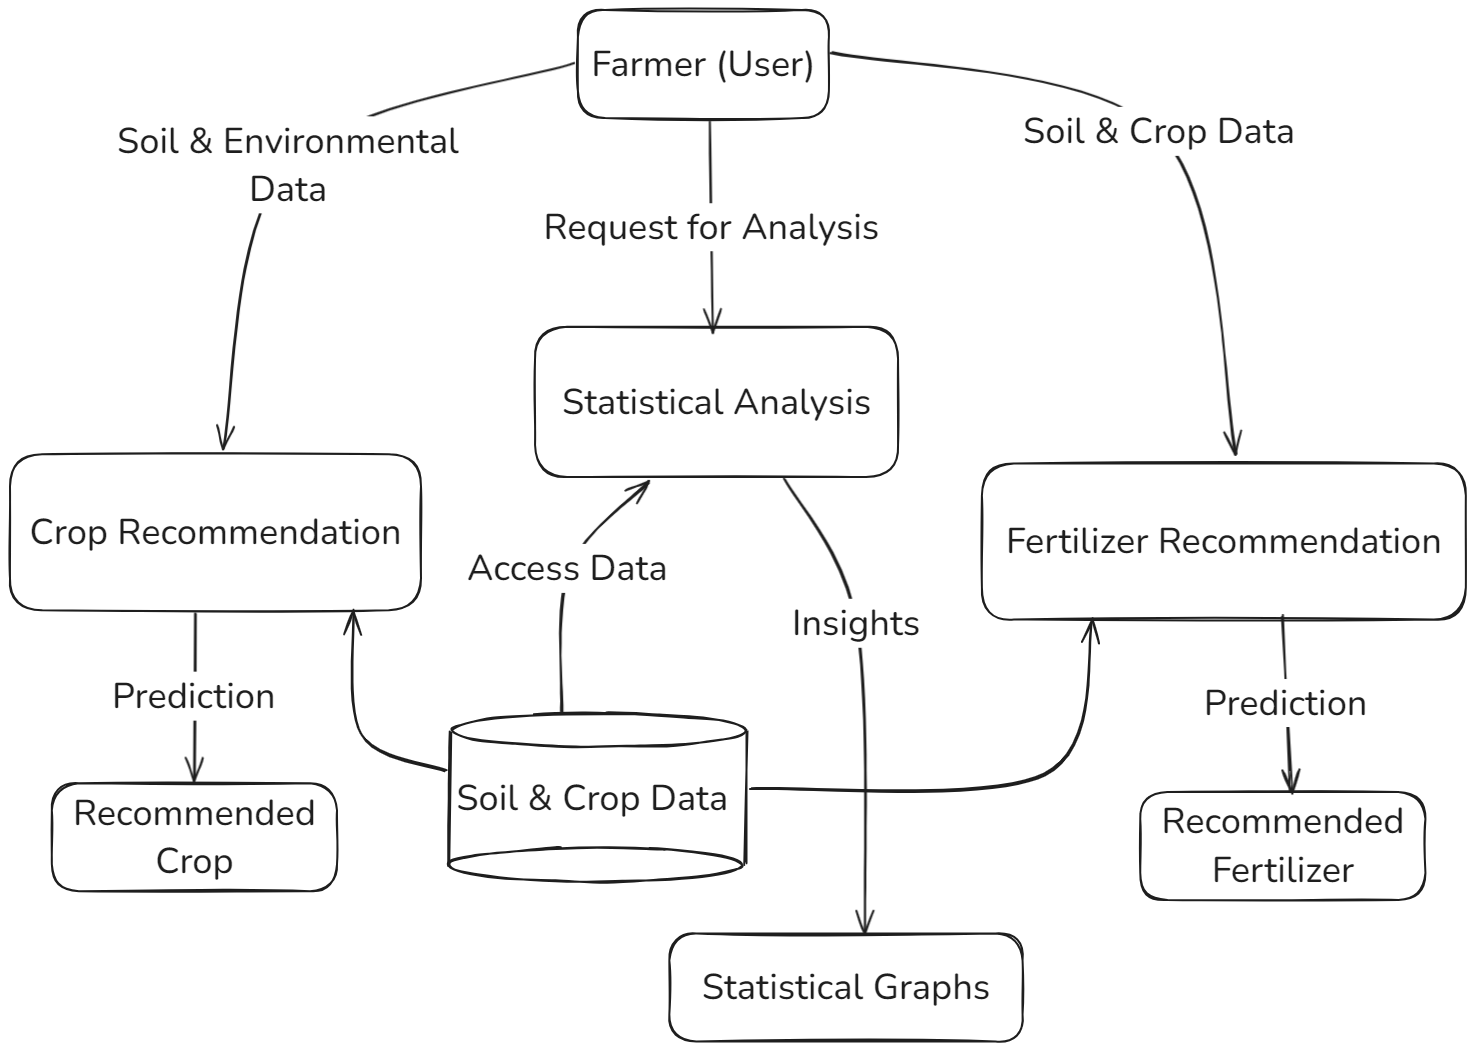
\includegraphics[width=10cm]{Entire_Flow_Diagram.png}
%     \caption{Entire work-flow of FarmSathi}
%     \label{fig:FarmSathi}
% \end{figure}

\textbf{The entire Work-flow} illustrates the main functional interactions:  
\begin{enumerate}
    \item Farmers provide \textit{soil and environmental data} as inputs to the system.
    \item The \textit{Crop Recommendation Module} predicts the best crops based on the inputs.
    \item The \textit{Fertilizer Recommendation Module} suggests fertilizers tailored to the selected crop and soil conditions.
    \item The \textit{Statistical Analysis Module} generates graphical insights to support sustainable farming practices.
\end{enumerate}
\newline
\textbf{System Workflow}: The database interacts with the crop and fertilizer recommendation models to retrieve relevant data, process inputs, and generate accurate outputs. Insights from the statistical analysis module further enhance the system's utility.  
\newline
This workflow ensures that all entities are interconnected and that the system delivers actionable, precise, and sustainable solutions for modern farming.  

\chapter{Overall Description}

\section{Product Perspective}
The "FarmSathi" system is a modern solution aimed at helping farmers make informed decisions by providing crop and fertilizer recommendations based on various environmental and soil conditions. Traditionally, farmers used manual methods for selecting crops and fertilizers, relying on limited data and experience. This website-based application aims to streamline that process by utilizing machine learning algorithms to suggest optimal farming choices. The primary goal of this project is to improve agricultural efficiency by minimizing guesswork and maximizing crop yield.

\section{User Classes and Characteristics}
"FarmSathi" has three primary types of users:
\begin{itemize}
    \item Registered Users (Farmers who use the system to input soil and climate data and receive recommendations)
    \item Admin (Responsible for managing user accounts and ensuring proper data is entered)
\end{itemize}
Farmers are the primary users who input data related to their fields, including soil conditions, climate, and historical crop performance. Agricultural experts can provide additional insights and updates to recommendations based on changing trends and data. System administrators manage the website's backend, ensuring the smooth operation of the platform.

% \begin{figure}[h!]
%     \centering
%     \includegraphics[width=10cm]{2.JPG}
%     \caption{Types of Users}
%     \label{fig:type of users}
% \end{figure}

\section{Product Functions}
The "FarmSathi" system will allow farmers to input various data points related to their fields, including soil type, pH, moisture levels, and climate conditions. Based on this input, the system will provide crop and fertilizer recommendations optimized for those specific conditions.
\newpage

The main functions of the system are as follows:
\begin{itemize}
    \item User Registration and Authentication
    \item Soil and Climate Data Input
    \item Crop and Fertilizer Recommendations
    \item Result Display (including expected crop yield and required care)
    \item Notifications and Alerts related to field care
\end{itemize}
\newline
All users have basic information stored in the system such as username, email, and role (e.g., Farmer, Expert, Admin). The system will maintain detailed profiles for each user, storing their input data for continuous updates and improvements in recommendations.
\newline
Each user type will have different access levels, such as:
\begin{itemize}
        \item Farmers can input data and view recommendations.
        \item Agricultural Experts can update the database with insights.
        \item Administrators have full access to manage users, data, and system settings.
    \end{itemize}

% \begin{figure}[h!]
%     \centering
%     \includegraphics[width=15cm]{3.JPG}
%     \caption{Data Flow Diagram}
%     \label{fig:Data Flow Diagram}
% \end{figure}

\section{Operating Environment}
The "FarmSathi" website will be designed to operate on multiple operating systems, including Mac, Windows, and Linux. The application will be hosted on a cloud server, making it accessible via any modern web browser, ensuring accessibility for farmers in rural areas with minimal technical infrastructure.

\section{Design}
The Farmer Activities are as follows:
\begin{itemize}
    \item Register on the website
    \item Input soil and environmental data
    \item Receive crop and fertilizer recommendations
    \item View detailed results, including expected yield and required farming practices
    \item Receive notifications regarding crop care and updates
\end{itemize}

\chapter{System Features}

\section{User Registration and Authentication}
\textbf{Description and Priority:} \newline 
Farmers and other users can register and log in to the FarmSathi application to access crop and fertilizer recommendations. This feature is of \textbf{High} priority.
\newline

\textbf{Stimulus/Response Sequences:}  
\begin{enumerate}
    \item User opens the application.
    \item User selects "Register" or "Login."
    \item User enters credentials.
    \item System verifies credentials and grants access.
\end{enumerate}

\textbf{Functional Requirements:}  
\begin{itemize}
    \item REQ-1: The system shall allow users to register using their email or phone number.
    \item REQ-2: The system shall verify user credentials during login.
    \item REQ-3: The system shall provide options for password recovery.
    \item REQ-4: The system shall implement multi-factor authentication for enhanced security.
\end{itemize}

\section{Crop Recommendation}
Description and Priority:  
FarmSathi provides farmers with recommendations on the most suitable crops based on environmental and soil data. This feature is of \textbf{High} priority.
\newline

\textbf{Stimulus/Response Sequences:}  
\begin{enumerate}
    \item User inputs soil data (e.g., nitrogen, phosphorus, potassium levels, pH, and moisture).
    \item User inputs environmental data (e.g., temperature and humidity).
    \item System processes the input data and predicts the optimal crop.
\end{enumerate}

\textbf{Functional Requirements:}  
\begin{itemize}
    \item REQ-5: The system shall accept soil and environmental parameters as input.
    \item REQ-6: The system shall use the trained logistic regression model for crop prediction.
    \item REQ-7: The system shall provide a list of top recommended crops based on input data.
\end{itemize}

\section{Fertilizer Recommendation}
Description and Priority:  
FarmSathi recommends appropriate fertilizers based on the soil's nutrient levels and crop type. This feature is of \textbf{High} priority.
\newline

\textbf{Stimulus/Response Sequences:}  
\begin{enumerate}
    \item User inputs soil nutrient levels (e.g., nitrogen, phosphorus, potassium).
    \item User selects the crop type.
    \item System processes the input data and suggests an optimal fertilizer.
\end{enumerate}

\textbf{Functional Requirements:}  
\begin{itemize}
    \item REQ-8: The system shall accept soil nutrient levels and crop type as input.
    \item REQ-9: The system shall use the trained random forest model for fertilizer prediction.
    \item REQ-10: The system shall display detailed fertilizer suggestions and their benefits.
\end{itemize}

\section{Data Visualization and Insights}
Description and Priority:  
The system provides visual insights into soil and crop data trends, enabling farmers to make informed decisions. This feature is of \textbf{Medium} priority.
\newline

 \textbf{Stimulus/Response Sequences: }
\begin{enumerate}
    \item User selects "View Insights."
    \item System processes stored data and generates visualizations (e.g., bar graphs, pie charts).
    \item User views insights to understand crop performance and soil trends.
\end{enumerate}
\newpage
\textbf{Functional Requirements: } 
\begin{itemize}
    \item REQ-11: The system shall generate graphs showing trends in soil nutrient levels and crop performance.
    \item REQ-12: The system shall display data comparisons across multiple crops and fertilizers.
    \item REQ-13: The system shall provide downloadable reports of the insights.
\end{itemize}


\section{System Administration}
\subsection{Description and Priority}
Administrators manage user accounts, monitor the database, and update the recommendation models. This feature is of \textbf{Medium} priority.
\subsection{Stimulus/Response Sequences}
\begin{enumerate}
    \item Administrator logs into the system.
    \item Administrator reviews user data and system logs.
    \item Administrator updates machine learning models and manages the database.
\end{enumerate}
\subsection{Functional Requirements}
\begin{itemize}
    \item REQ-14: The system shall allow administrators to create and manage user accounts.
    \item REQ-15: The system shall provide logs for monitoring user activity and system performance.
    \item REQ-16: The system shall allow administrators to update machine learning models as needed.
\end{itemize}

\section{Customer Support}
\subsection{Description and Priority}
Users can access help and support for resolving issues related to the FarmSathi application. This feature is of \textbf{Medium} priority.
\subsection{Stimulus/Response Sequences}
\begin{enumerate}
    \item User selects "Help and Support."
    \item User describes the issue or selects a predefined query.
    \item System provides a solution or connects the user to support staff.
\end{enumerate}
\subsection{Functional Requirements}
\begin{itemize}
    \item REQ-17: The system shall provide a FAQ section for common issues.
    \item REQ-18: The system shall allow users to contact customer support via email or chat.
    \item REQ-19: The system shall allow users to report technical issues directly through the app.
\end{itemize}

\chapter{Other Nonfunctional Requirements}

\section{Performance Requirements}
"FarmSathi" is designed to operate efficiently under varying user loads, ensuring a seamless experience for farmers and agricultural experts. Key performance considerations include:
\begin{itemize}
    \item The system must provide crop and fertilizer recommendations within 2-3 seconds of input submission.
    \item Handle concurrent user requests without significant delays, supporting at least 100 simultaneous users.
    \item Optimize database queries to ensure real-time insights and predictions.
\end{itemize}

\section{Security Requirements}
"FarmSathi" ensures data integrity and user privacy through robust security measures:
\begin{itemize}
    \item Only authenticated users can access the system, with role-based permissions ensuring farmers, agricultural experts, and administrators perform their designated actions.
    \item User data and recommendations are encrypted both in transit and at rest to prevent unauthorized access.
    \item Regular security audits to identify vulnerabilities and strengthen defenses against threats.
\end{itemize}

\section{Software Quality Attributes}
The following quality attributes are critical for the success of "FarmSathi":
\begin{itemize}
    \item \textbf{Reliability:} The system must function without failure during critical agricultural seasons.
    \item \textbf{Usability:} A user-friendly interface with intuitive navigation ensures easy adoption by farmers.
    \item \textbf{Scalability:} Designed to accommodate additional features, datasets, and an increasing number of users in the future.
    \item \textbf{Maintainability:} Modular code structure to simplify updates and bug fixes.
    \item \textbf{Testability:} Comprehensive testing, including database validation, logic checks, and UI testing, is conducted to ensure functionality.
\end{itemize}

\section{Business Rules}
"FarmSathi" follows business rules aimed at promoting sustainable farming practices:
\begin{itemize}
    \item The system exclusively recommends crops and fertilizers suited to the provided soil and environmental data to maximize productivity.
    \item Statistical analysis tools are integrated to help farmers understand the rationale behind recommendations.
    \item Updates to the database are allowed only by authenticated administrators or agricultural experts, ensuring data accuracy and relevance.
    \item Data insights are aligned with regional agricultural guidelines to support localized farming needs.
\end{itemize}

\chapter{Other Requirements}

"FarmSathi" requires ongoing maintenance to adapt to evolving agricultural practices and technological advancements. 

\section{System Maintenance:} 
    \begin{itemize}
        \item Regular updates to the database to include new crop varieties, fertilizers, and soil data.
        \item Periodic optimization of machine learning models to maintain accuracy as new data becomes available.
        \item Bug fixes and performance enhancements to ensure smooth operation.
    \end{itemize}
\section{Future Scalability:} 
    \begin{itemize}
        \item Integration of additional features such as pest management, irrigation recommendations, and weather predictions.
        \item Expansion to support multi-language interfaces to cater to diverse user demographics.
        \item Compatibility with mobile platforms for wider accessibility.
    \end{itemize}
\section{User Training and Support:}
    \begin{itemize}
        \item Development of training modules to educate farmers on using the platform effectively.
        \item Providing a dedicated helpdesk or chatbot for addressing user queries and technical issues.
    \end{itemize}
\section{Compliance and Updates:} 
    \begin{itemize}
        \item Ensure compliance with regional agricultural regulations and data privacy laws.
        \item Regular updates based on user feedback and evolving industry standards.
    \end{itemize}


"FarmSathi" is designed to grow with its users and the agriculture sector, ensuring long-term usability and relevance.

\chapter{Appendix A: Glossary}
\begin{itemize}
    \item \textbf{Farmer:} A primary user of the system who provides soil, crop, and environmental data to receive crop and fertilizer recommendations.
    \item \textbf{Soil Type:} Classification of soil based on physical and chemical properties (e.g., Sandy, Loamy, Clayey).
    \item \textbf{Crop Recommendation System:} A module that predicts suitable crops for a specific region based on input data.
    \item \textbf{Fertilizer Recommendation System:} A module that suggests the most suitable fertilizer based on soil and crop data.
    \item \textbf{Random Forest:} A machine learning algorithm used for making accurate predictions in the fertilizer recommendation model.
    \item \textbf{Logistic Regression:} A machine learning algorithm employed for crop recommendation due to its interpretability and accuracy.
    \item \textbf{Environmental Factors:} Data like temperature, humidity, and rainfall affecting crop growth and fertilizer requirements.
    \item \textbf{Streamlit:} A Python-based framework used for developing and deploying the web application.
    \item \textbf{Azure Document Intelligence API:} A cloud-based OCR tool used for extracting soil test data from documents.
    \item \textbf{EDA (Exploratory Data Analysis):} The process of visualizing and summarizing data trends and relationships.
    \item \textbf{User-Friendly Interface:} A simple and intuitive interface enabling users to interact with the system effectively.
\end{itemize}

\chapter{Appendix B: Analysis Models}
\begin{figure}[h!]
    \centering
    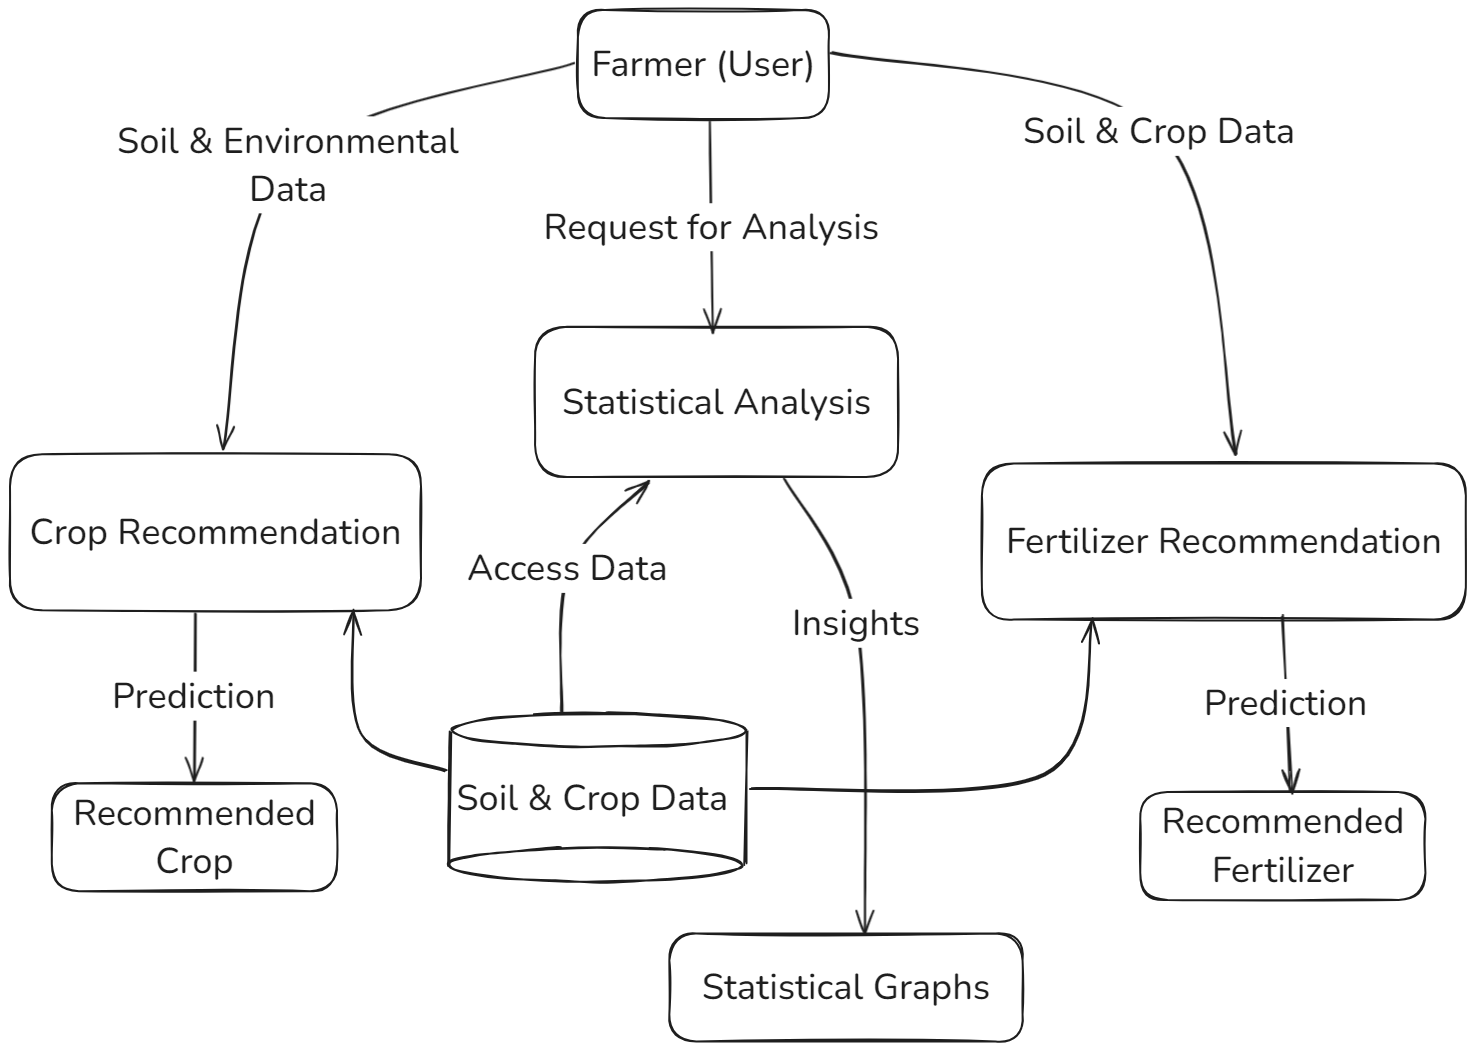
\includegraphics[width=0.6\linewidth]{Entire_Flow_Diagram.png}
    \caption{Work-flow Diagram of FarmSathi}
    \label{fig:FarmSathi_Workflow}
    
    \vspace{1cm}

    \centering
    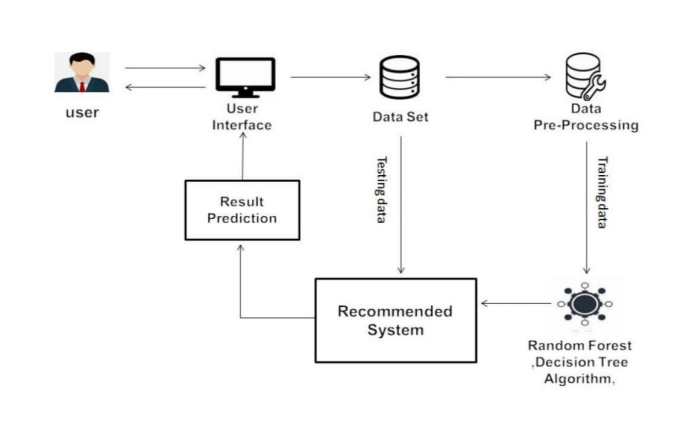
\includegraphics[width=0.8\linewidth]{System Architecture.png}
    \caption{System Architechture of FarmSathi}
    \label{fig:FarmSathi_Sysytem_Architecture}
\end{figure}

\begin{figure}
    \centering
    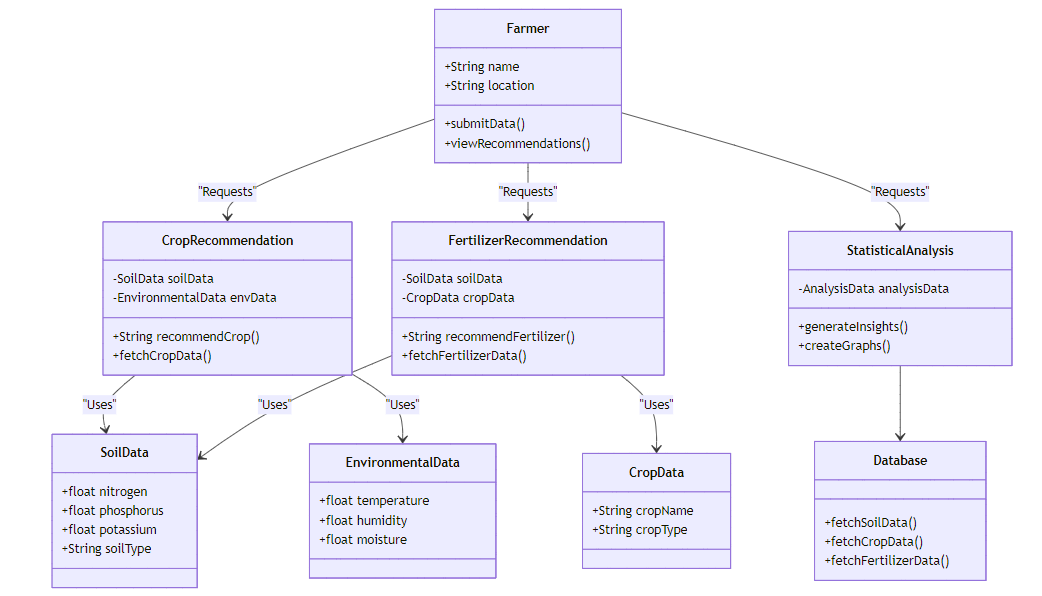
\includegraphics[width=1.0\linewidth]{Class Diagram.png}
    \caption{Class Diagram of FarmSathi}
    \label{fig:FarmSathi_Class}
    \vspace{1cm}
    \centering
    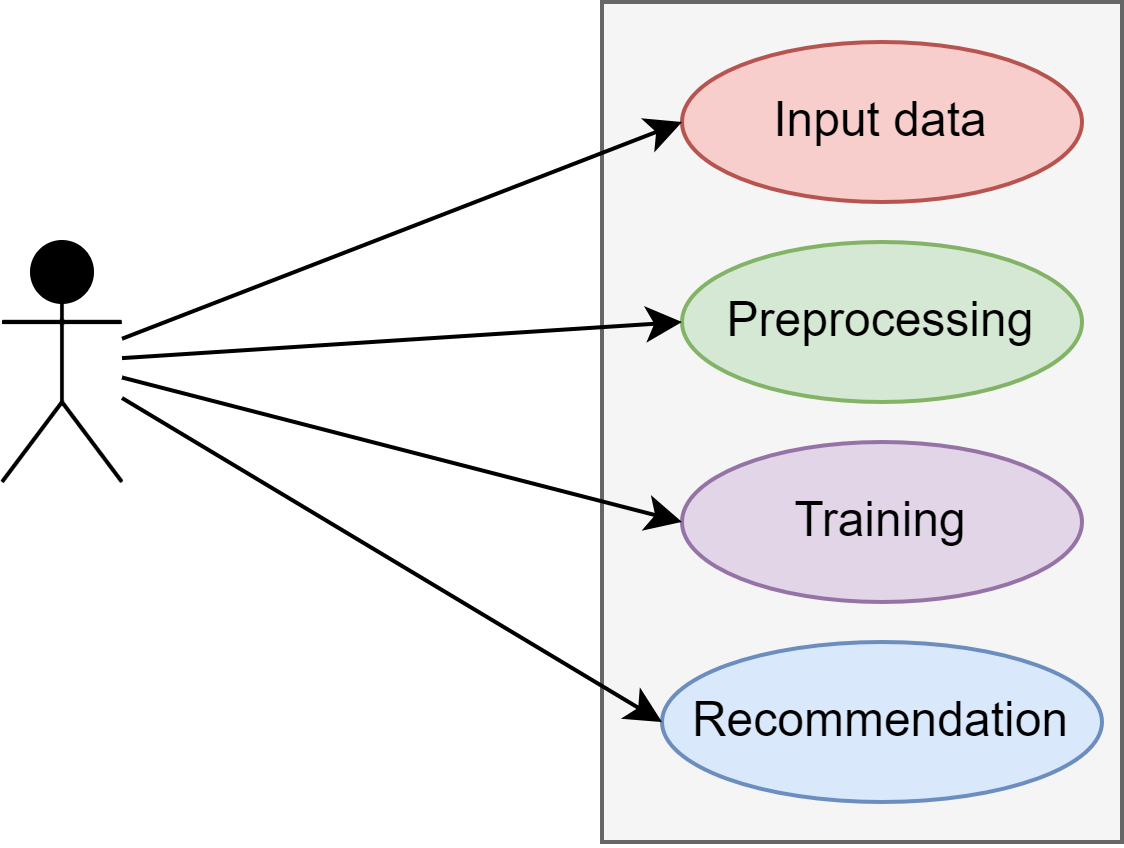
\includegraphics[width=0.5\linewidth]{Use_Case_Diagram.png}
    \caption{Use Case Diagram of FarmSathi}
    \label{fig:FarmSathi_Use_Case}
\end{figure}

\begin{figure}
    \centering
    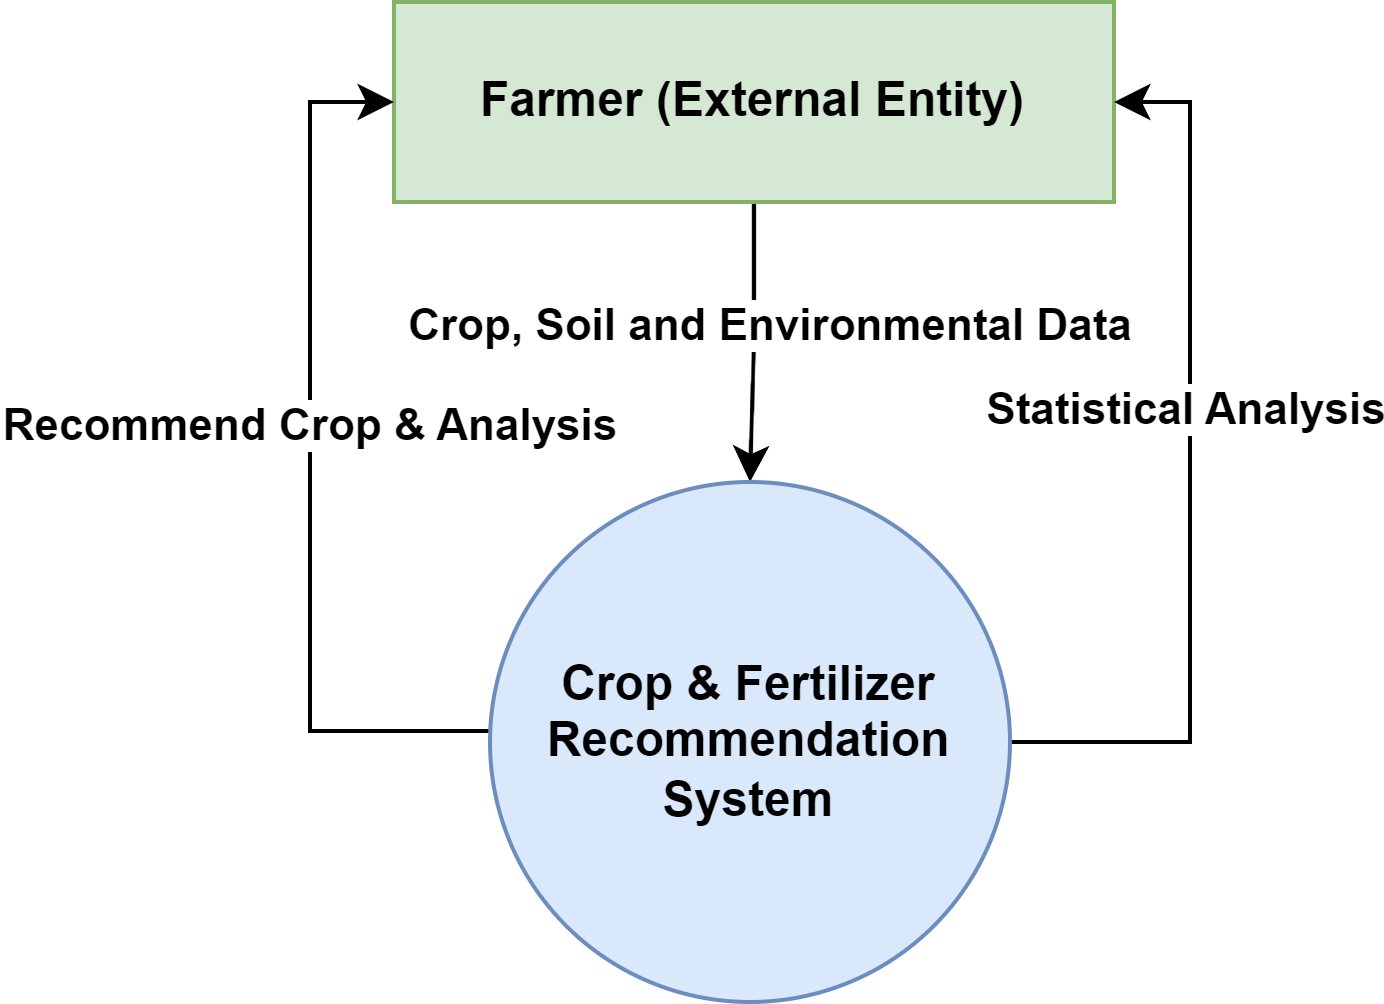
\includegraphics[width=0.7\linewidth]{Level_0_DFD.png}
    \caption{Level-0 Data Flow Diagram of FarmSathi}
    \label{fig:FarmSathi_DFD0}
    
    \vspace{1cm}
    
    \centering
    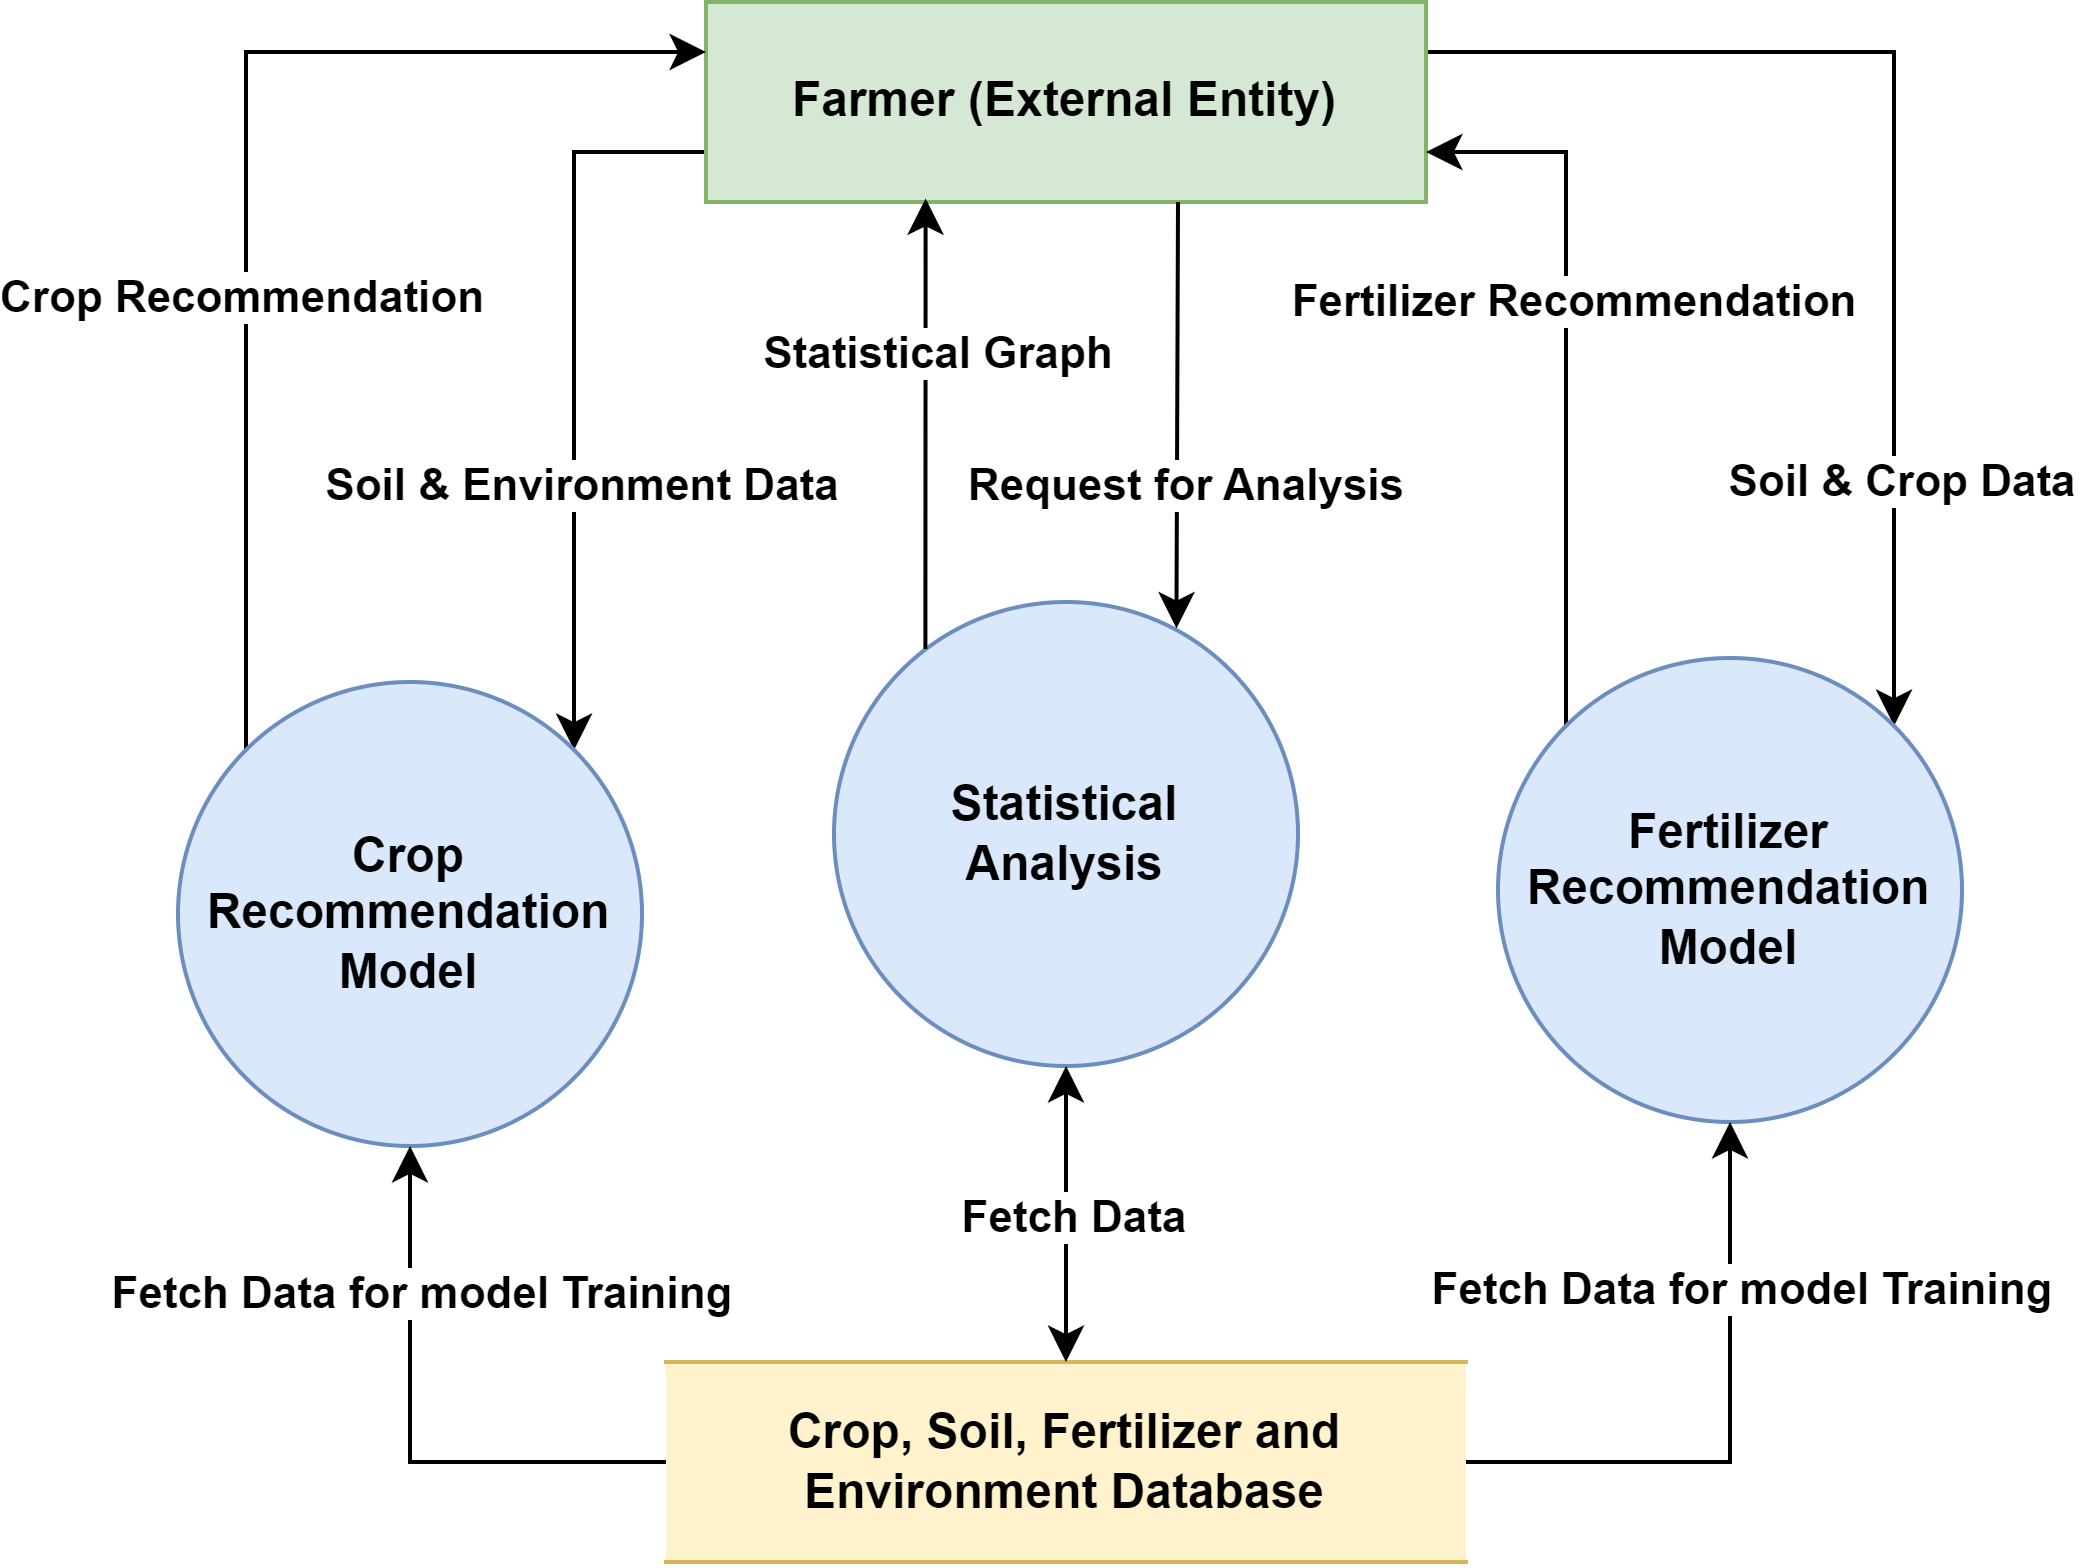
\includegraphics[width=1\linewidth]{Level_1_DFD.png}
    \caption{Level-1 Data Flow Diagram of FarmSathi}
    \label{fig:FarmSathi_DFD1}
    
\end{figure}

\chapter{Appendix C: To Be Determined List}
\begin{itemize}
    \item \textbf{TBD-1:} Integration of weather prediction data for better recommendations.
    \item \textbf{TBD-2:} Expansion to support pest management and irrigation suggestions.
    \item \textbf{TBD-3:} Additional language support for wider accessibility.
    \item \textbf{TBD-4:} Detailed analytics for agricultural trends and forecasting.
    \item \textbf{TBD-5:} Mobile platform optimization for real-time data input.
    \item \textbf{TBD-6:} Advanced visualization features for statistical insights.
    \item \textbf{TBD-7:} Integration with government and agricultural databases.
    \item \textbf{TBD-8:} Enhanced security features for sensitive user data.
    \item \textbf{TBD-9:} Customizable recommendations based on user feedback.
    \item \textbf{TBD-10:} AI-based model improvements for continuous learning and accuracy.
    \item \textbf{TBD-11:} Integration with third-party APIs for data enrichment.
    \item \textbf{TBD-12:} Regular testing and validation protocols for long-term reliability.
\end{itemize}

\end{document}